% This file was created by tikzplotlib v0.9.2.
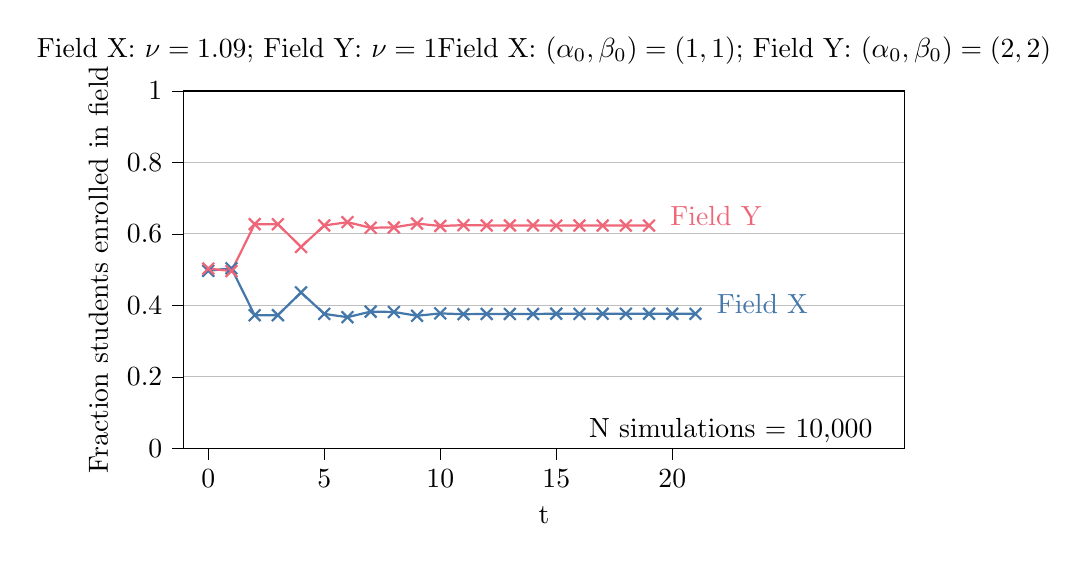
\begin{tikzpicture}

\definecolor{color0}{rgb}{0.266666666666667,0.466666666666667,0.666666666666667}
\definecolor{color1}{rgb}{0.933333333333333,0.4,0.466666666666667}

\begin{axis}[
height=6.121302808757603cm,
tick align=outside,
tick pos=left,
title={Field X: \(\displaystyle \nu = 1.09\); Field Y: \(\displaystyle \nu = 1\) \\ Field X: \(\displaystyle (\alpha_{0}, \beta_{0}) = (1, 1)\); Field Y: \(\displaystyle (\alpha_{0}, \beta_{0}) = (2, 2)\)},
unbounded coords=jump,
width=10.729849cm,
x grid style={white!69.0196078431373!black},
xlabel={t},
xmin=-1.05, xmax=30,
xtick style={color=black},
xtick={0,5,10,15,20},
xticklabels={\(\displaystyle 0\),\(\displaystyle 5\),\(\displaystyle 10\),\(\displaystyle 15\),\(\displaystyle 20\)},
ylabel={Fraction students enrolled in field},
ymajorgrids,
ymin=0, ymax=1,
ytick style={color=black},
ytick={0,0.2,0.4,0.6,0.8,1},
yticklabels={\(\displaystyle 0\),\(\displaystyle 0.2\),\(\displaystyle 0.4\),\(\displaystyle 0.6\),\(\displaystyle 0.8\),\(\displaystyle 1\)}
]
\addplot [thick, color0, mark=x, mark size=3, mark options={solid}]
table {%
0 0.4969
1 0.5039
2 0.3726
3 0.3728
4 0.4364
5 0.3763
6 0.3671
7 0.3827
8 0.3817
9 0.3711
10 0.3777
11 0.3754
12 0.3762
13 0.3762
14 0.3761
15 0.3768
16 0.3764
17 0.3766
18 0.3766
19 0.3767
20 0.3767
21 0.3766
};
\addplot [thick, color1, mark=x, mark size=3, mark options={solid}]
table {%
0 0.5031
1 0.4961
2 0.6274
3 0.6272
4 0.5636
5 0.6237
6 0.6329
7 0.6173
8 0.6183
9 0.6289
10 0.6223
11 0.6246
12 0.6238
13 0.6238
14 0.6239
15 0.6232
16 0.6236
17 0.6234
18 0.6234
19 0.6233
20 nan
21 nan
};
\draw (axis cs:21.5,0.3766) node[
  anchor=base west,
  text=color0,
  rotate=0.0
]{Field X};
\draw (axis cs:19.5,0.6233) node[
  anchor=base west,
  text=color1,
  rotate=0.0
]{Field Y};
\draw (axis cs:16,0.03) node[
  anchor=base west,
  text=black,
  rotate=0.0
]{N simulations = 10,000};
\end{axis}

\end{tikzpicture}
